\documentclass[aspectratio=169]{beamer}\usepackage[]{graphicx}\usepackage[]{color}
% maxwidth is the original width if it is less than linewidth
% otherwise use linewidth (to make sure the graphics do not exceed the margin)
\makeatletter
\def\maxwidth{ %
  \ifdim\Gin@nat@width>\linewidth
    \linewidth
  \else
    \Gin@nat@width
  \fi
}
\makeatother

\definecolor{fgcolor}{rgb}{0.345, 0.345, 0.345}
\newcommand{\hlnum}[1]{\textcolor[rgb]{0.686,0.059,0.569}{#1}}%
\newcommand{\hlstr}[1]{\textcolor[rgb]{0.192,0.494,0.8}{#1}}%
\newcommand{\hlcom}[1]{\textcolor[rgb]{0.678,0.584,0.686}{\textit{#1}}}%
\newcommand{\hlopt}[1]{\textcolor[rgb]{0,0,0}{#1}}%
\newcommand{\hlstd}[1]{\textcolor[rgb]{0.345,0.345,0.345}{#1}}%
\newcommand{\hlkwa}[1]{\textcolor[rgb]{0.161,0.373,0.58}{\textbf{#1}}}%
\newcommand{\hlkwb}[1]{\textcolor[rgb]{0.69,0.353,0.396}{#1}}%
\newcommand{\hlkwc}[1]{\textcolor[rgb]{0.333,0.667,0.333}{#1}}%
\newcommand{\hlkwd}[1]{\textcolor[rgb]{0.737,0.353,0.396}{\textbf{#1}}}%
\let\hlipl\hlkwb

\usepackage{framed}
\makeatletter
\newenvironment{kframe}{%
 \def\at@end@of@kframe{}%
 \ifinner\ifhmode%
  \def\at@end@of@kframe{\end{minipage}}%
  \begin{minipage}{\columnwidth}%
 \fi\fi%
 \def\FrameCommand##1{\hskip\@totalleftmargin \hskip-\fboxsep
 \colorbox{shadecolor}{##1}\hskip-\fboxsep
     % There is no \\@totalrightmargin, so:
     \hskip-\linewidth \hskip-\@totalleftmargin \hskip\columnwidth}%
 \MakeFramed {\advance\hsize-\width
   \@totalleftmargin\z@ \linewidth\hsize
   \@setminipage}}%
 {\par\unskip\endMakeFramed%
 \at@end@of@kframe}
\makeatother

\definecolor{shadecolor}{rgb}{.97, .97, .97}
\definecolor{messagecolor}{rgb}{0, 0, 0}
\definecolor{warningcolor}{rgb}{1, 0, 1}
\definecolor{errorcolor}{rgb}{1, 0, 0}
\newenvironment{knitrout}{}{} % an empty environment to be redefined in TeX

\usepackage{alltt}
\usepackage{multirow}
%\usecolortheme{beaver}
%\usecolortheme[RGB={129,3,3}]{structure}
\usetheme{CambridgeUS}
\usecolortheme{seahorse}

% Standard header (will need to change date!)
\title[GEOG 5680 Summer '20]{GEOG 5680\\Introduction to R}
\subtitle[Intro]{10: Statistical modeling in R}
\author[S. Brewer]{Simon Brewer}
\institute[Univ. Utah]{
  Geography Department\\
  University of Utah\\
  Salt Lake City, Utah 84112\\[1ex]
  \texttt{simon.brewer@geog.utah.edu}
}
\date[May 05, 2020]{May 05, 2020}
\IfFileExists{upquote.sty}{\usepackage{upquote}}{}
\begin{document}


%--- the titlepage frame -------------------------%
\begin{frame}
  \titlepage
\end{frame}

% \section{Objectives}
% %--- Slide 3 ----------------%
% \begin{frame}{Objectives}
% \begin{itemize}
%   \item Introduce statistical modeling in R
%   \item Look at the formula syntax
%   \item Model diagnostics
% \end{itemize}
% \end{frame}
% 
\section{Statistical modeling}
%--- Slide ----------------%
\begin{frame}{Statistical modeling}
Data = predictable component + unpredictable component
\begin{equation}
  y = f + \epsilon
\end{equation}
\begin{itemize}
	\item Interest in understanding the function $f$ which explains observations ($y$): 
	\begin{itemize}
	  \item should explain as much variation as possible
	\end{itemize}
	\item The unpredictable part is also important: 
	\begin{itemize}
	  \item should be random noise (i.e. nothing left that we can explain)
	\end{itemize}
	\item Used for \emph{understanding process} and \emph{prediction}
\end{itemize}
\end{frame}

%--- Slide ----------------%
\begin{frame}{A Simple Model}
\begin{columns}
  \begin{column}{0.5\textwidth}
		\begin{itemize}
			\item Consumption of ice cream
			\item Simplest model is just $E(y) = \mu$
			\item With unexplained variance described by a normal distribution $N(0, \sigma^2)$
			% \item For a normally distributed dataset ($E(y) = N(\mu,\sigma^2$))
		\end{itemize}
	\end{column}
	\begin{column}{0.5\textwidth}
\begin{knitrout}\scriptsize
\definecolor{shadecolor}{rgb}{0.969, 0.969, 0.969}\color{fgcolor}
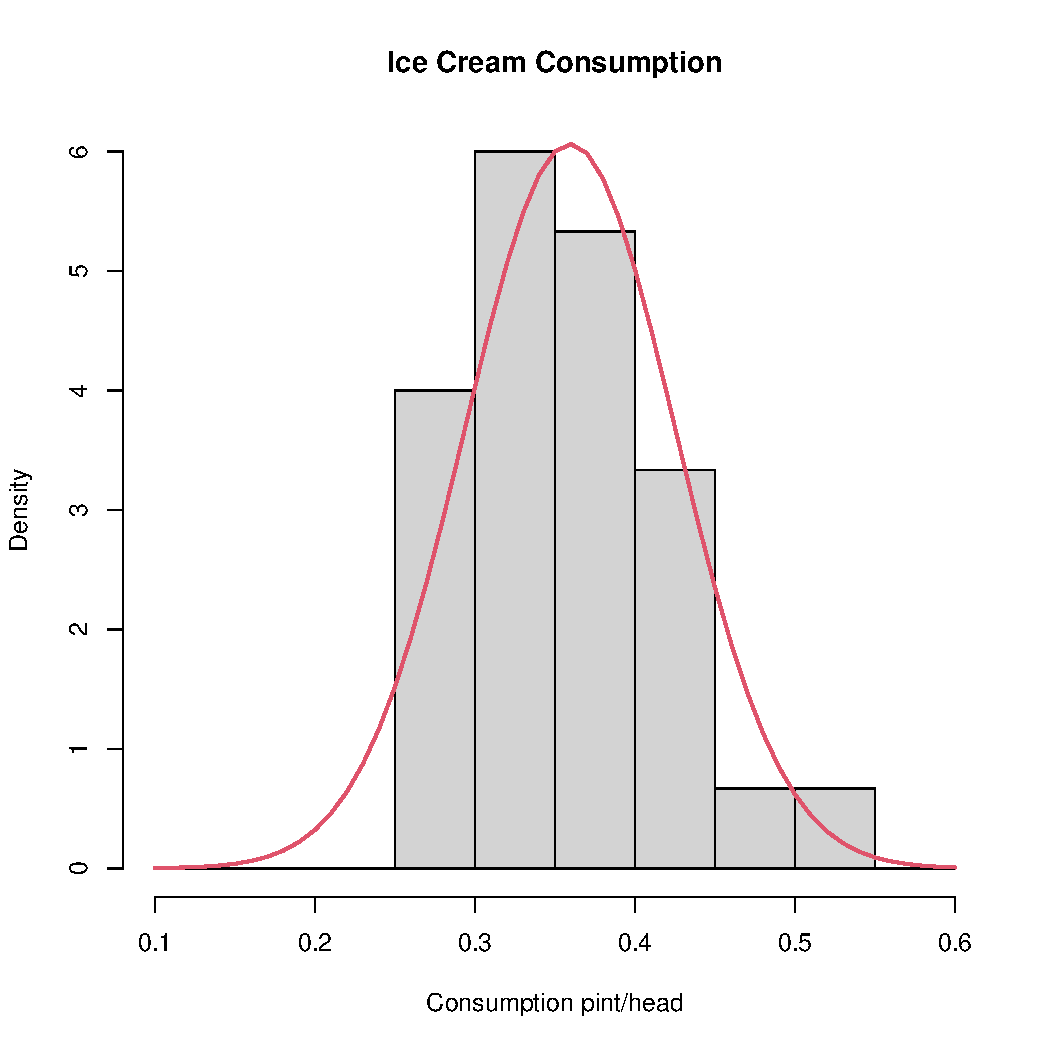
\includegraphics[width=\maxwidth]{figure/unnamed-chunk-1-1} 

\end{knitrout}
\end{column}
\end{columns}
\end{frame}

%--- Slide ----------------%
\begin{frame}{A Simple Model}
\begin{columns}
  \begin{column}{0.5\textwidth}
		\begin{itemize}
			\item Most statistical modeling introduces independent variables
			\item Can we improve on simple model by introducing $x$? 
			\item E.g. daily temperature
			\item Expected value ($E(y|x) = \beta_0 + \beta_1 x + \epsilon$)
			\item Where $\epsilon = N(0, \sigma^2$)
		\end{itemize}
	\end{column}
	\begin{column}{0.5\textwidth}
\begin{knitrout}\scriptsize
\definecolor{shadecolor}{rgb}{0.969, 0.969, 0.969}\color{fgcolor}
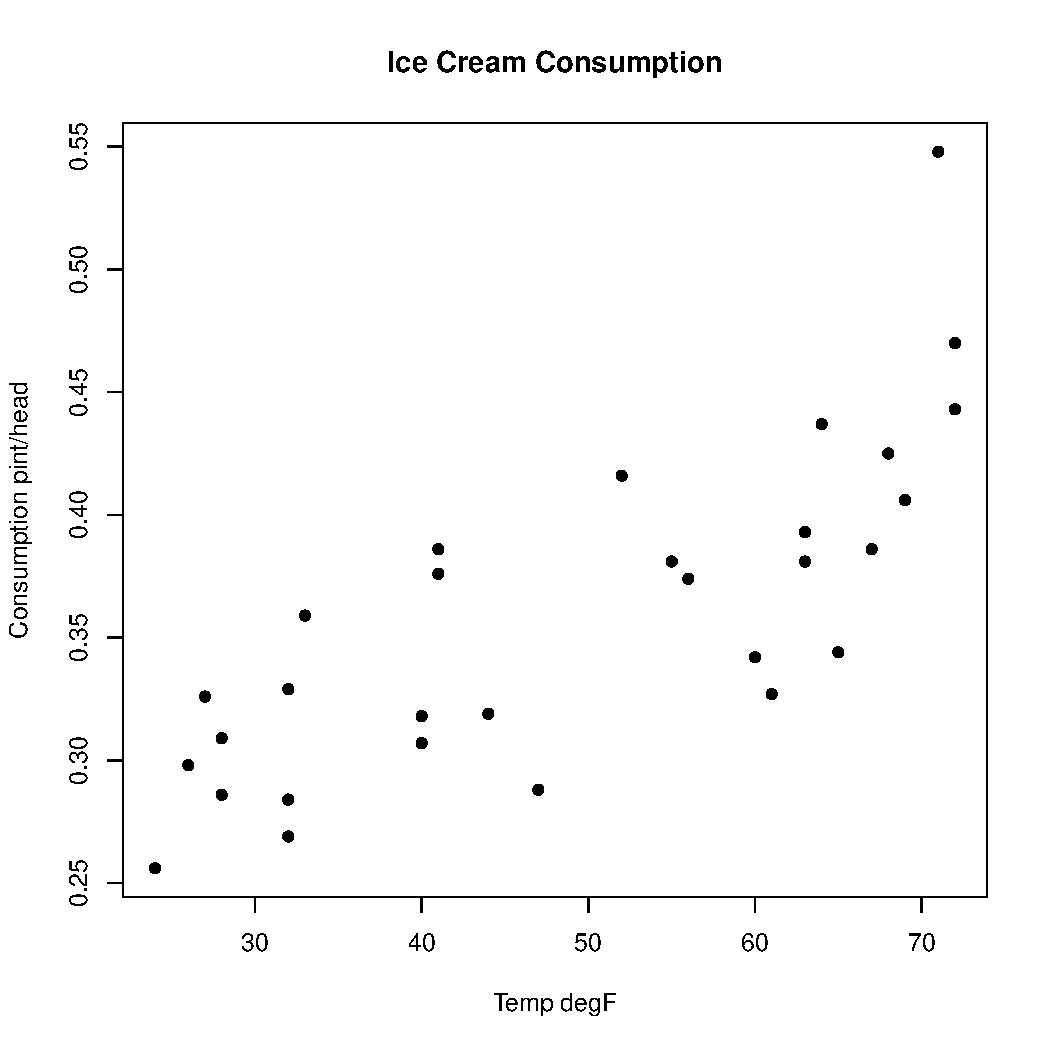
\includegraphics[width=\maxwidth]{figure/unnamed-chunk-2-1} 

\end{knitrout}
\end{column}
\end{columns}
\end{frame}

%' %--- Slide ----------------%
%' \begin{frame}{A Simple Model}
%' \begin{columns}
%'   \begin{column}{0.5\textwidth}
%' 		\begin{itemize}
%' 			\item Consumption is the response, temperature is the explanatory variable
%' 			\item Can test this with correlations but we are also interested in the strength (slope) of the relationship (the \textit{rate} of change)
%' 		\end{itemize}
%' 	\end{column}
%' 	\begin{column}{0.5\textwidth}
%' <<echo=FALSE>>=
%' Icecream<-read.csv("icecream.csv")
%' plot(Icecream$cons ~ Icecream$temp, xlab='Temp degF', ylab='Consumption pint/head', pch=16, main='Ice Cream Consumption')
%' fit = lm(cons ~ temp, data=Icecream)
%' abline(fit, col=2, lwd=3)
%' @
%' \end{column}
%' \end{columns}
%' \end{frame}

%--- Slide ----------------%
\begin{frame}[fragile]{A Simple Model}
\begin{columns}
	\begin{column}{0.5\textwidth}
		\begin{itemize}
			\item Simple linear regression fit by minimizing the sum of squares (distance between observed and modeled $y$)
			\item The slope gives the strength of the relationship (the \emph{rate} of change)
			\item The intercept is expected value of $y$ at $x=0$
		\end{itemize}
	\end{column}
	\begin{column}{0.5\textwidth}
\begin{knitrout}\scriptsize
\definecolor{shadecolor}{rgb}{0.969, 0.969, 0.969}\color{fgcolor}
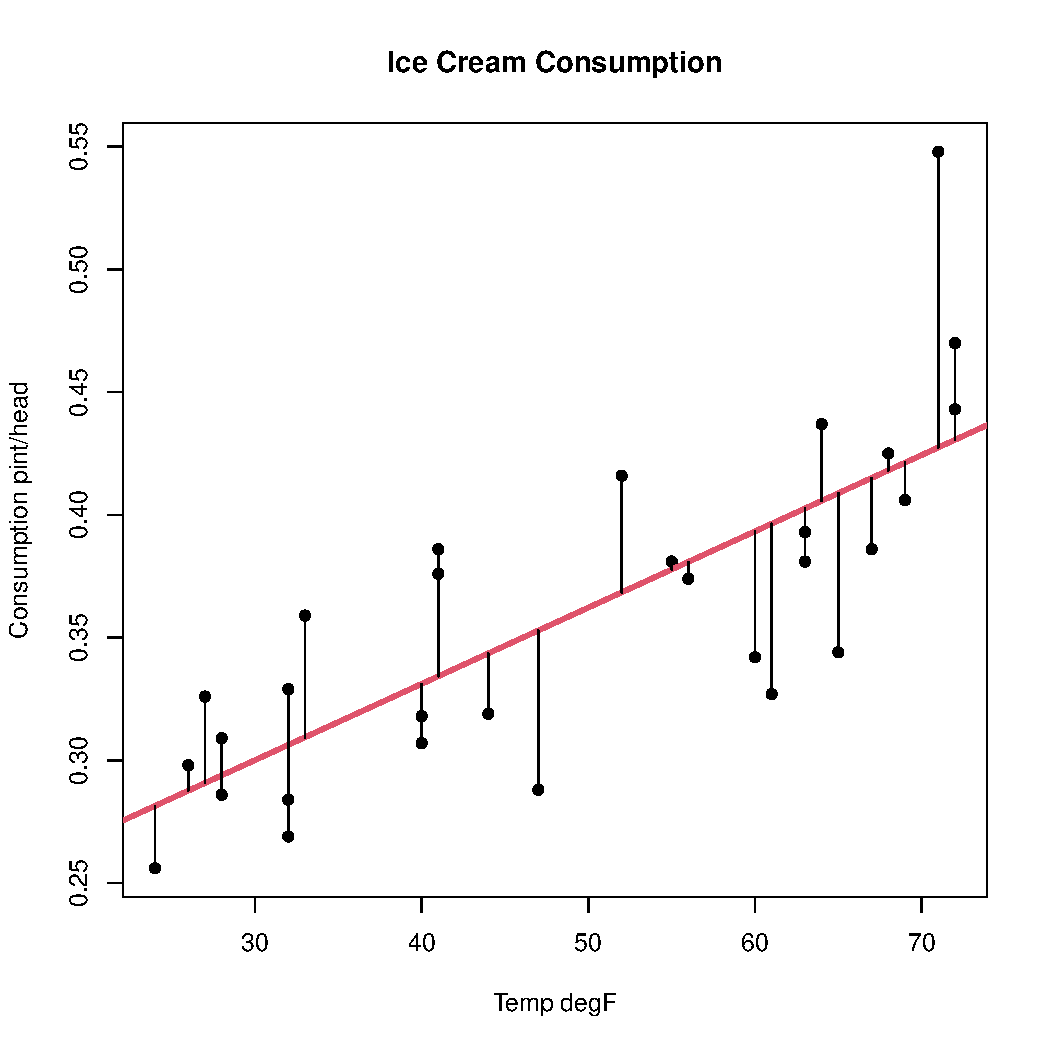
\includegraphics[width=\maxwidth]{figure/unnamed-chunk-3-1} 

\end{knitrout}
	\end{column}
\end{columns}
\end{frame}

%--- Slide ----------------%
\begin{frame}[fragile]{Linear models in R}
R syntax --- 'formula' method uses the \emph{tilde} ($\sim$)
\begin{itemize}
	\item Dependent variable on left, explanatory variable(s) on right: \texttt{lm($y \sim x_1 + x_2 \ldots$)}
	\item Model fitting produces a model \emph{object} as output, so create a variable to store this:
\end{itemize}
\begin{knitrout}\scriptsize
\definecolor{shadecolor}{rgb}{0.969, 0.969, 0.969}\color{fgcolor}\begin{kframe}
\begin{alltt}
\hlstd{fit} \hlkwb{=} \hlkwd{lm}\hlstd{(cons} \hlopt{~} \hlstd{temp, Icecream)}
\hlstd{fit}
\end{alltt}
\begin{verbatim}
## 
## Call:
## lm(formula = cons ~ temp, data = Icecream)
## 
## Coefficients:
## (Intercept)         temp  
##    0.206862     0.003107
\end{verbatim}
\end{kframe}
\end{knitrout}
\end{frame}

%--- Slide ----------------%
\begin{frame}[fragile]{Centering data}
\begin{itemize}
	\item If the value of $x=0$ is not meaningful, we can center the data by subtracting the mean from covariates
	\item $x_{i,cen} = x_i - \bar{x}$
\end{itemize}
\begin{knitrout}\scriptsize
\definecolor{shadecolor}{rgb}{0.969, 0.969, 0.969}\color{fgcolor}\begin{kframe}
\begin{alltt}
\hlstd{Icecream}\hlopt{$}\hlstd{temp.c} \hlkwb{=} \hlstd{Icecream}\hlopt{$}\hlstd{temp} \hlopt{-} \hlkwd{mean}\hlstd{(Icecream}\hlopt{$}\hlstd{temp)}
\hlstd{fit} \hlkwb{=} \hlkwd{lm}\hlstd{(cons} \hlopt{~} \hlstd{temp.c, Icecream)}
\hlstd{fit}
\end{alltt}
\begin{verbatim}
## 
## Call:
## lm(formula = cons ~ temp.c, data = Icecream)
## 
## Coefficients:
## (Intercept)       temp.c  
##    0.359433     0.003107
\end{verbatim}
\end{kframe}
\end{knitrout}
\end{frame}

\section{Diagnostics}
%--- Slide ----------------%
\begin{frame}{Diagnostics}
\begin{itemize}
  \item Coefficients
  \item Goodness of fit
	\begin{itemize}
		\item ANOVA
		\item $F$-statistic
		\item $r$-squared: variance explained
	\end{itemize}
	\item Residuals and diagnostic plots
	\item These ideas can be applied to most models
\end{itemize}
\end{frame}

%--- Slide ----------------%
\begin{frame}[fragile]{R Model Diagnostics}
\begin{knitrout}\scriptsize
\definecolor{shadecolor}{rgb}{0.969, 0.969, 0.969}\color{fgcolor}\begin{kframe}
\begin{alltt}
\hlkwd{summary}\hlstd{(fit)}
\end{alltt}
\begin{verbatim}
## 
## Call:
## lm(formula = cons ~ temp.c, data = Icecream)
## 
## Residuals:
##       Min        1Q    Median        3Q       Max 
## -0.069411 -0.024478 -0.007371  0.029126  0.120516 
## 
## Coefficients:
##              Estimate Std. Error t value Pr(>|t|)    
## (Intercept) 0.3594333  0.0077159  46.584  < 2e-16 ***
## temp.c      0.0031074  0.0004779   6.502 4.79e-07 ***
## ---
## Signif. codes:  0 '***' 0.001 '**' 0.01 '*' 0.05 '.' 0.1 ' ' 1
## 
## Residual standard error: 0.04226 on 28 degrees of freedom
## Multiple R-squared:  0.6016,	Adjusted R-squared:  0.5874 
## F-statistic: 42.28 on 1 and 28 DF,  p-value: 4.789e-07
\end{verbatim}
\end{kframe}
\end{knitrout}
\begin{itemize}
\item Note the use of the summary function with a \emph{model} object. 
\end{itemize}
\end{frame}

\subsection{ANOVA}
% %--- Slide ----------------%
% \begin{frame}{ANOVA}
% Decomposition of variance for a dataset with three groups
%   \begin{center}
% 		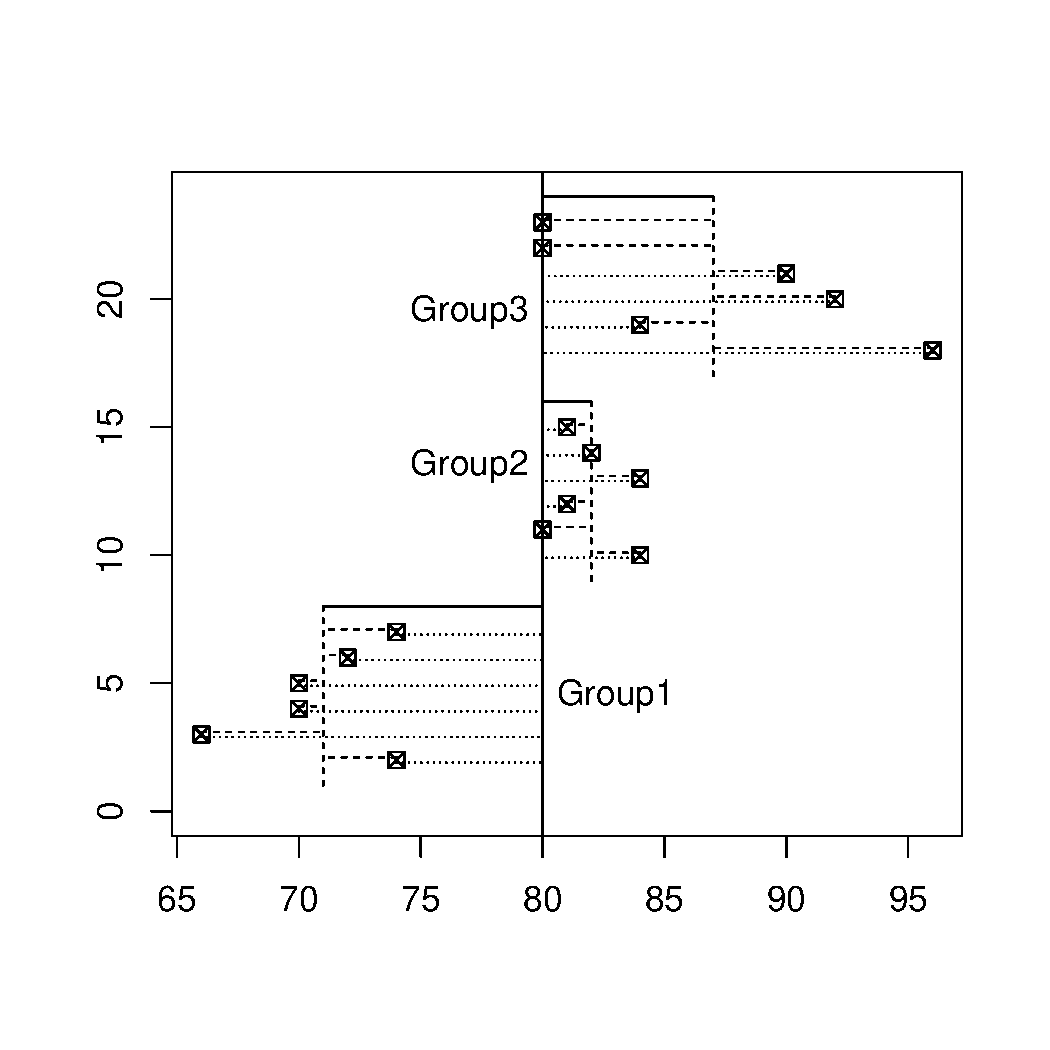
\includegraphics[width=0.6\textwidth]{./images/sourcesofvariance}
% 	\end{center}
% \end{frame}
% 
% %--- Slide ----------------%
% \begin{frame}{ANOVA}
% We now square and sum the differences for each observations as follow
% \begin{equation}
% 	\sum_{i=1}^{t} \sum_{j=1}^{n} (x_{ij} - \bar{x})^2 = 
% 	n \sum_{i=1}^{t} (\bar{x_i} - \bar{x})^2 + 
% 	\sum_{i=1}^{t} \sum_{j=1}^{n} (x_{ij} - \bar{x_i})^2
% \end{equation}
% \emph{Total} variation or \emph{sum of squares} may be split into \emph{between} and
% \emph{error} components\\
% Frequently written as:
% \begin{equation}
% 	TSS = BSS + ESS
% \end{equation}
% \end{frame}
% 
% %--- Slide ----------------%
% \begin{frame}{ANOVA}
% The $F$-statistic is used to test for significance in the split of variance:
% \begin{equation}
% 		F = \frac{BSS/t(n-1)}{ESS/t} 
% \end{equation}
% \begin{itemize}
% 	\item Ratio of how much of the variance is between the groups to how much is within the groups
% 	\item Compare to an $F$-distribution, using degrees of freedom based on the number of groups and the number of observations
% \end{itemize}
% \end{frame}
% 
% %--- Slide ----------------%
% \begin{frame}{ANOVA with a linear model}
% Model variance can be split into sums of squares components --- Total (TSS), Model (MSS), Error/Residual (RSS)
% \begin{equation}
%   RSS = \sum_{i=1}^n(y_i - \hat{y_i})^2
% \end{equation}
% \begin{equation}
% 	MSS = \sum_{i=1}^n(\bar{y_i} - \hat{y_i})^2
% \end{equation}
% \begin{equation}
% 	TSS = \sum_{i=1}^n(y_i - \bar{y_i})^2 = RSS + MSS
% \end{equation}
% A good model will explain a large proportion of the TSS in the MSS
% \end{frame}

%--- Slide ----------------%
\begin{frame}{ANOVA}
ANOVA can be used to test model goodness-of-fit
\begin{equation}
		F = \frac{MSS/(df1)}{RSS/(df2)} 
\end{equation}
\begin{itemize}
	\item Ratio of how much of the variance is explained by the model (MSS) to the variance in the residuals (RSS)
	\item Compare to an $F$-distribution, using degrees of freedom based on the number of parameters and the number of observations
\end{itemize}
\end{frame}

%--- Slide ----------------%
\begin{frame}[fragile]{ANOVA with a linear model}
\begin{columns}
  \begin{column}{0.33\textwidth}
		Total SS

\begin{knitrout}\scriptsize
\definecolor{shadecolor}{rgb}{0.969, 0.969, 0.969}\color{fgcolor}
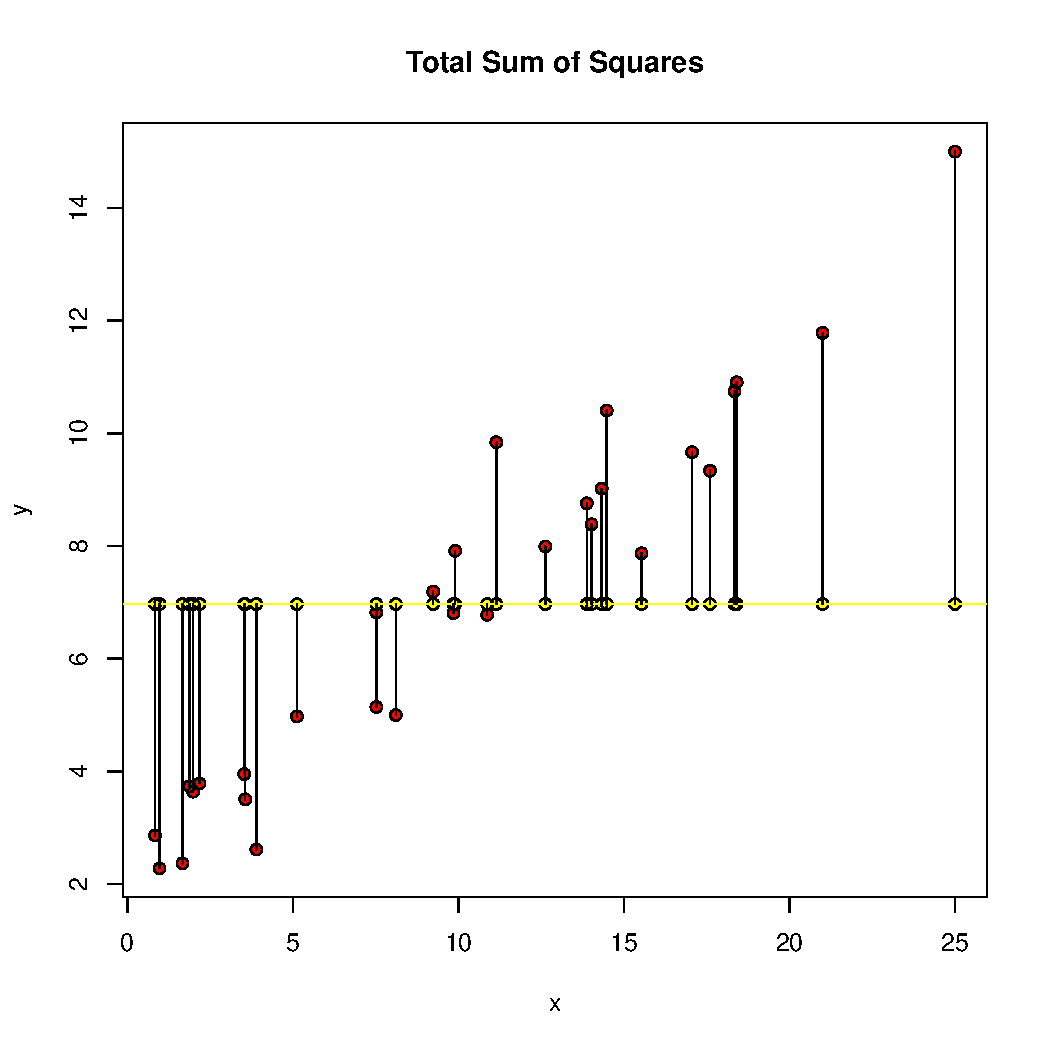
\includegraphics[width=\maxwidth]{figure/unnamed-chunk-8-1} 

\end{knitrout}
	\end{column}
	\begin{column}{0.33\textwidth}
		Residual SS
\begin{knitrout}\scriptsize
\definecolor{shadecolor}{rgb}{0.969, 0.969, 0.969}\color{fgcolor}
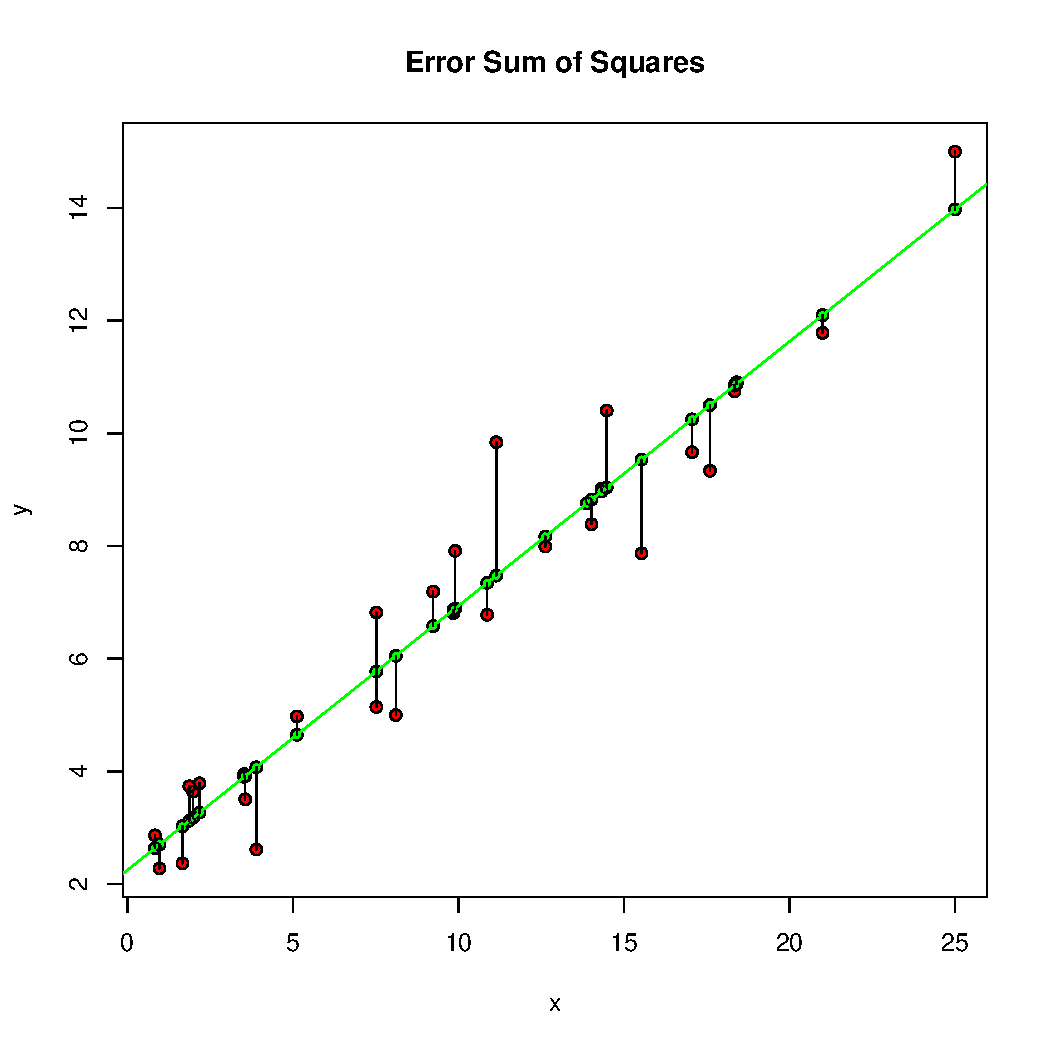
\includegraphics[width=\maxwidth]{figure/unnamed-chunk-9-1} 

\end{knitrout}
\end{column}
	\begin{column}{0.33\textwidth}
		Model SS
\begin{knitrout}\scriptsize
\definecolor{shadecolor}{rgb}{0.969, 0.969, 0.969}\color{fgcolor}
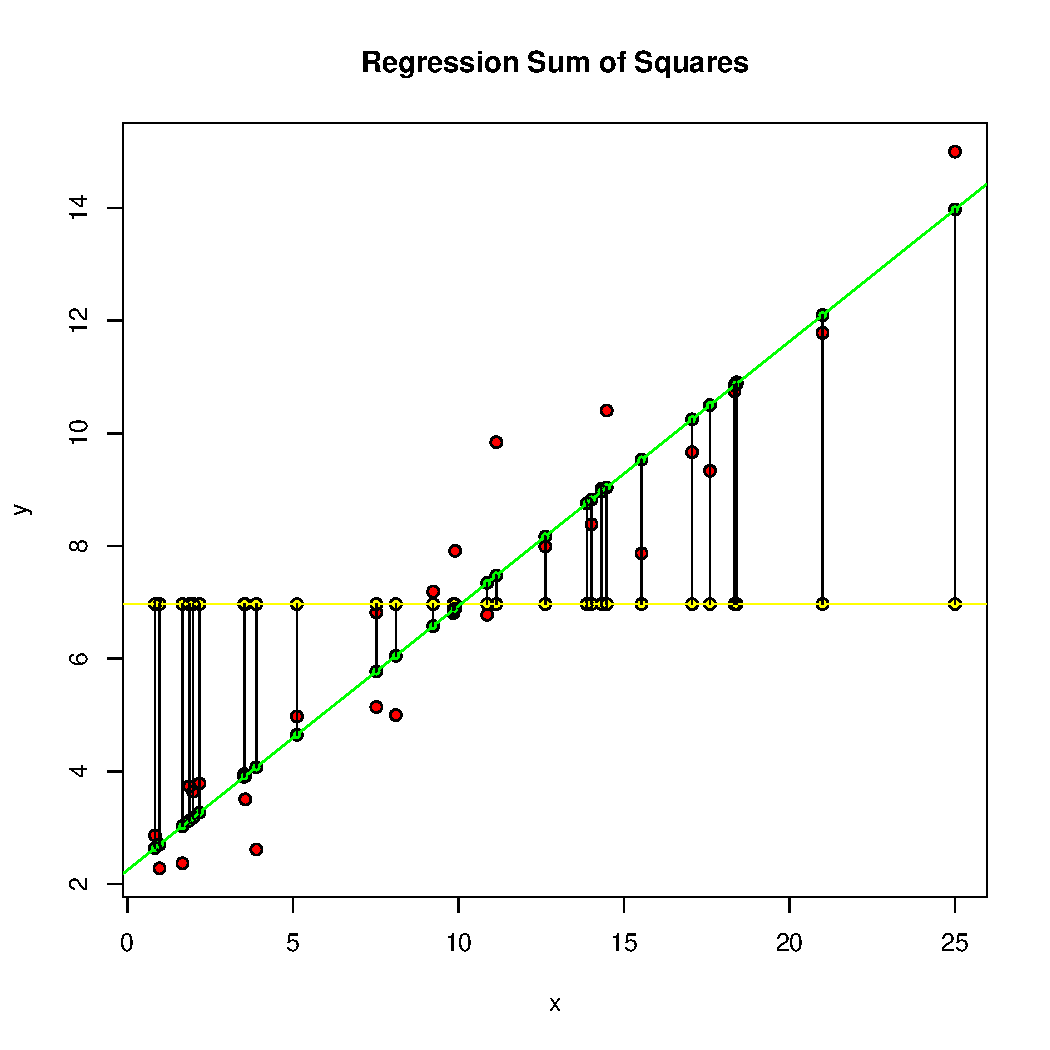
\includegraphics[width=\maxwidth]{figure/unnamed-chunk-10-1} 

\end{knitrout}
	\end{column}
\end{columns}
\end{frame}

% %--- Slide ----------------%
% \begin{frame}{ANOVA with a linear model}
% Note that this partitioning of variance (Total, Model, Residual) is the same procedure as when calculating an ANOVA. \\
% Linear model:
% \begin{equation}
% 	TSS 	= 	MSS	+ RSS		
% \end{equation}
% ANOVA:
% \begin{equation}
% 	TSS		=	BSS 	+ ESS
% \end{equation}
% \begin{itemize}
%   \item Rather than using groups to explain the variance, we use the regression model
%   \item We can then use ANOVA to analyze the variance explained by our regression model
% \end{itemize}
% \end{frame}
% 
%--- Slide ----------------%
\begin{frame}[fragile]{ANOVA with a linear model}
\begin{knitrout}\scriptsize
\definecolor{shadecolor}{rgb}{0.969, 0.969, 0.969}\color{fgcolor}\begin{kframe}
\begin{alltt}
\hlkwd{anova}\hlstd{(ex1.lm)}
\end{alltt}
\begin{verbatim}
## Analysis of Variance Table
## 
## Response: y
##           Df  Sum Sq Mean Sq F value    Pr(>F)    
## x          1 283.947 283.947   368.4 < 2.2e-16 ***
## Residuals 28  21.581   0.771                      
## ---
## Signif. codes:  0 '***' 0.001 '**' 0.01 '*' 0.05 '.' 0.1 ' ' 1
\end{verbatim}
\end{kframe}
\end{knitrout}
\end{frame}

\subsection{Residuals and Diagnostic Plots}
%--- Slide ----------------%
\begin{frame}{Residuals and Diagnostic Plots}
  \begin{itemize}
		\item Regression function can be wrong (quadratic or other effects)
		\item Model for the errors may be incorrect:
		\begin{itemize}
			\item may not be normally distributed.
			\item may not be independent.
			\item may not have the same variance.
		\end{itemize}
		\item If model is correct then residuals should resemble random variables with mean = 0 and a normal distribution
		\item Detecting problems is more art then science, i.e. we cannot test for all possible problems in a regression model.
	\end{itemize}
\end{frame}

%--- Slide ----------------%
\begin{frame}[fragile]{Residuals and Diagnostic Plots}
\begin{columns}
  \begin{column}{0.5\textwidth}
	\begin{itemize}
		\item Plot of residuals vs. fitted values
		\item Look for \emph{bias} in residuals to indicate a poor model fit
		\item Also use histograms, Q-Q plots, etc
	\end{itemize}
\begin{knitrout}\scriptsize
\definecolor{shadecolor}{rgb}{0.969, 0.969, 0.969}\color{fgcolor}\begin{kframe}
\begin{alltt}
\hlkwd{plot}\hlstd{(fit,} \hlkwc{which}\hlstd{=}\hlnum{1}\hlstd{)}
\end{alltt}
\end{kframe}
\end{knitrout}
  \end{column}
  \begin{column}{0.5\textwidth}
\begin{knitrout}\scriptsize
\definecolor{shadecolor}{rgb}{0.969, 0.969, 0.969}\color{fgcolor}
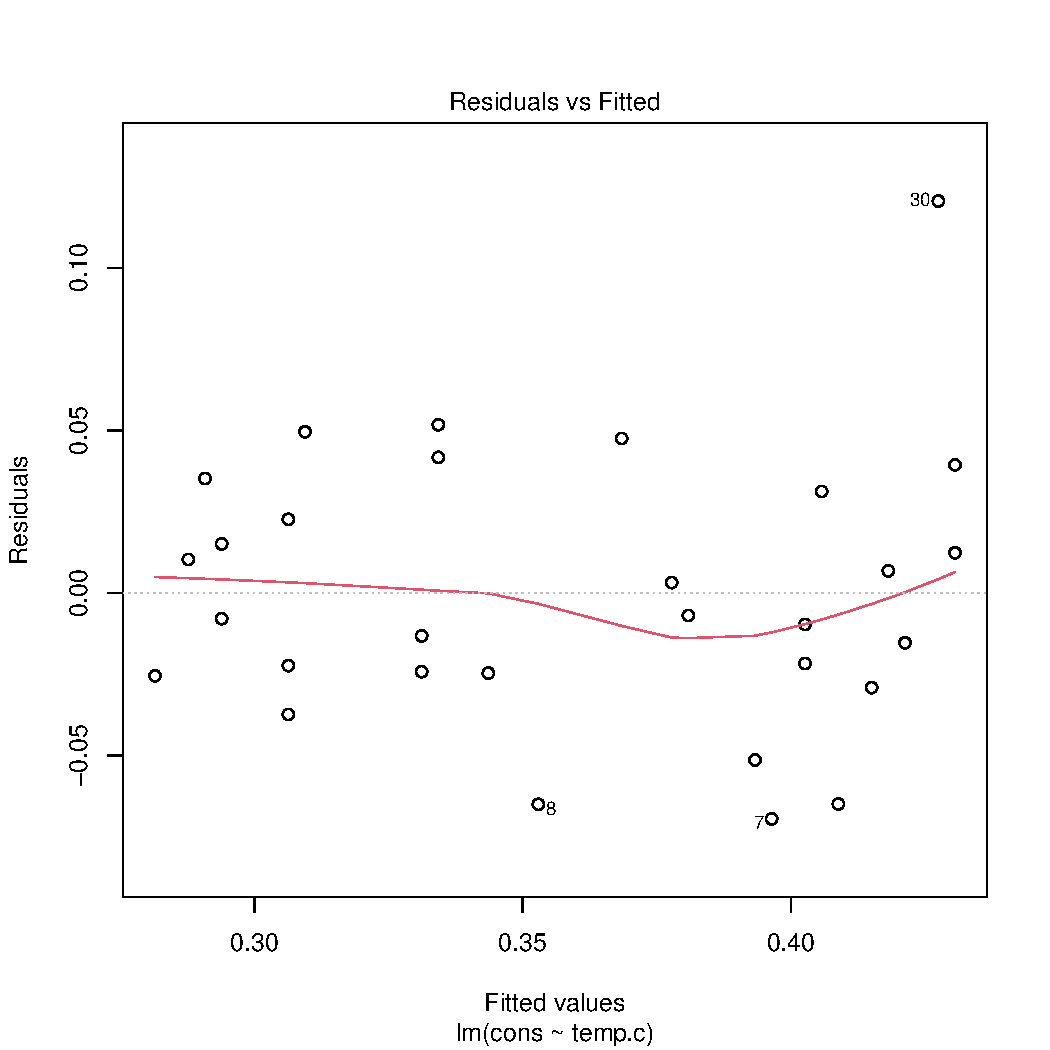
\includegraphics[width=\maxwidth]{figure/unnamed-chunk-13-1} 

\end{knitrout}
  \end{column}
\end{columns}
\end{frame}

%--- Slide ----------------%
\begin{frame}[fragile]{Residuals and Diagnostic Plots}
\begin{columns}
  \begin{column}{0.5\textwidth}
	\begin{itemize}
		\item Plot of Cook's distance
		\item Low if $x_i$ is close to other $x$'s
		\item High if $x_i$ is distant: indicates high leverage and influence in regression
	\end{itemize}
\begin{knitrout}\scriptsize
\definecolor{shadecolor}{rgb}{0.969, 0.969, 0.969}\color{fgcolor}\begin{kframe}
\begin{alltt}
\hlkwd{plot}\hlstd{(fit,} \hlkwc{which}\hlstd{=}\hlnum{4}\hlstd{)}
\end{alltt}
\end{kframe}
\end{knitrout}
  \end{column}
  \begin{column}{0.5\textwidth}
\begin{knitrout}\scriptsize
\definecolor{shadecolor}{rgb}{0.969, 0.969, 0.969}\color{fgcolor}
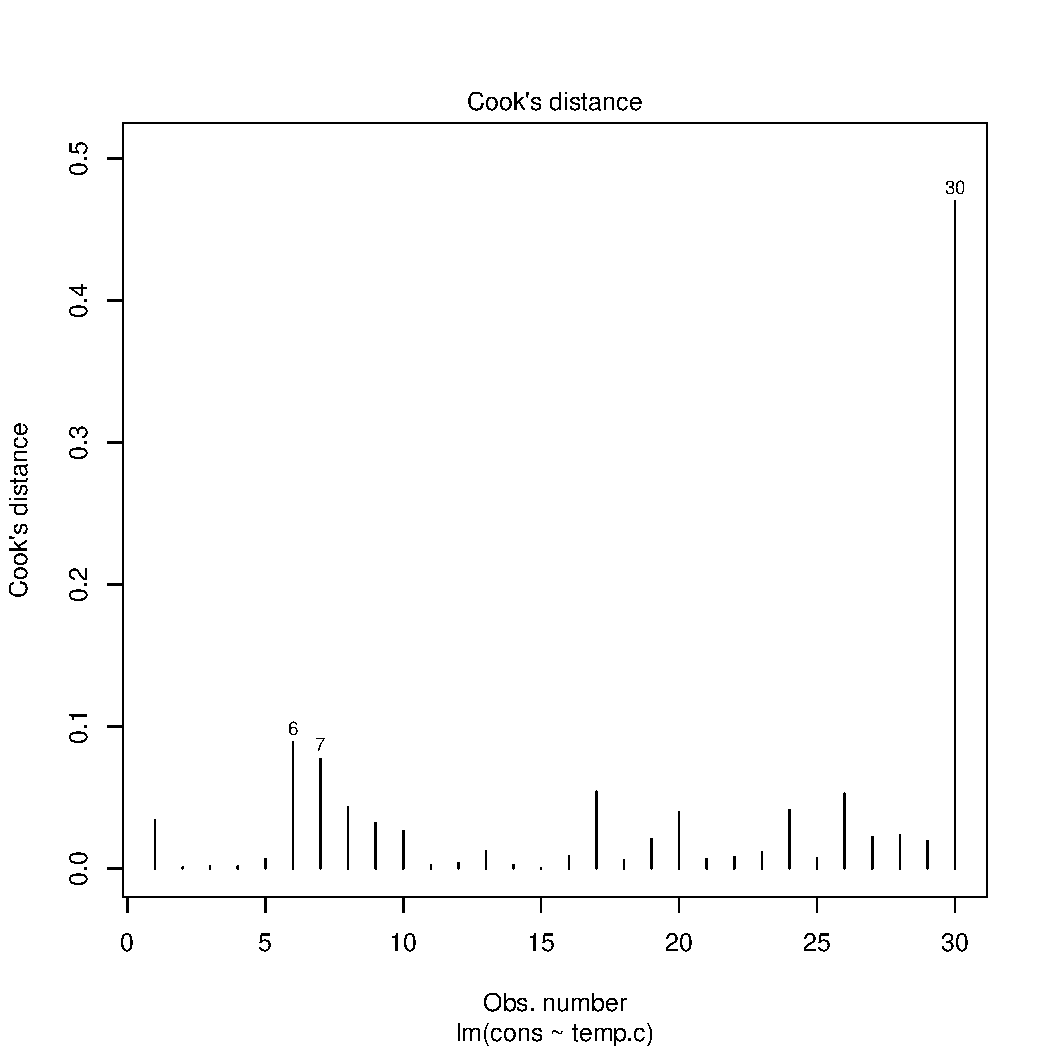
\includegraphics[width=\maxwidth]{figure/unnamed-chunk-15-1} 

\end{knitrout}
  \end{column}
\end{columns}
\end{frame}

\section{Predictions}
%--- Slide ----------------%
\begin{frame}[fragile]{Predictions}
\begin{itemize}
  \item Predicting for new values of $x$
  \item Requires new data frame containing variable(s) with the same name(s) as the independent $x$'s used in model
  \item \texttt{interval} parameter estimates 95\% prediction CIs
\end{itemize}
\begin{knitrout}\scriptsize
\definecolor{shadecolor}{rgb}{0.969, 0.969, 0.969}\color{fgcolor}\begin{kframe}
\begin{alltt}
\hlstd{newtemp} \hlkwb{=} \hlkwd{data.frame}\hlstd{(}\hlkwc{temp.c} \hlstd{=} \hlnum{70} \hlopt{-} \hlkwd{mean}\hlstd{(Icecream}\hlopt{$}\hlstd{temp))}
\hlkwd{predict}\hlstd{(fit,} \hlkwc{newdata} \hlstd{= newtemp,} \hlkwc{interval} \hlstd{=} \hlstr{"pred"}\hlstd{)}
\end{alltt}
\begin{verbatim}
##         fit     lwr       upr
## 1 0.4243771 0.33403 0.5147241
\end{verbatim}
\end{kframe}
\end{knitrout}
\end{frame}

\section{Extensions to basic model}
%--- Slide ----------------%
\begin{frame}{Extensions to basic model}
\begin{itemize}
  \item Multiple linear regression
  \item Dummy variables
  \item Interactions
  \item Generalized linear modeling
	\begin{itemize}
		\item Logistic regression
		\item Poisson regression
	\end{itemize}
	\item Many other non/semi-parametric, Bayesian and machine learning methods available
\end{itemize}
\end{frame}

% %--- Slide ----------------%
% \begin{frame}[fragile]{LOTR Actor Dataste}
% \begin{itemize}
%   \item Physical characteristics of actors auditioning for Lord of the Rings
% \end{itemize}
% <<echo=FALSE>>=
% lotr = read.csv("lotr_hw.csv")
% str(lotr)
% @
% \begin{itemize}
%   \item Subset of Aragorn actors:
% \end{itemize}
% <<echo=TRUE>>=
% aragorn <- subset(lotr, role=='Aragorn')
% @
% \end{frame}
% 
% \subsection{Multiple linear regression}
% %--- Slide ----------------%
% \begin{frame}[fragile]{Multiple linear regression}
% Initial height-weight model with subset of data
% <<echo=FALSE>>=
% aragorn = subset(lotr, role=="Aragorn")
% @
% <<>>=
% fit1 = lm(weight ~ height, aragorn)
% summary(fit1)
% @
% \end{frame}
% 
% % %--- Slide ----------------%
% % \begin{frame}[fragile]{LOTR Actor Dataset}
% % \begin{itemize}
% %   \item Intercept is round(coef(fit1)[1],4) --- for an actor of 0cm height
% %   \item Centering independent variable can improve interpretability 
% % \end{itemize}
% % <<>>=
% % aragorn$height.cen = aragorn$height - mean(aragorn$height)
% % fit1 = lm(weight ~ height.cen, aragorn)
% % fit1
% % @
% % \begin{itemize}
% %   \item Intercept is now round(coef(fit1)[1],2) --- for an actor of average height
% % \end{itemize}
% % \end{frame}
% % 
% %--- Slide ----------------%
% \begin{frame}[fragile]{Multiple linear regression}
% Model with multiple variables
% <<>>=
% fit2 = lm(weight ~ height + fachair, aragorn)
% summary(fit2)
% @
% \end{frame}
% 
% \begin{frame}[fragile]{Multiple linear regression}
% ANOVA to compare models
% <<>>=
% anova(fit1, fit2)
% @
% \end{frame}
% 
% \section{Dummy variables}
% %--- Slide ----------------%
% \begin{frame}{Dummy variables}
% \begin{itemize}
%   \item Including binary or categorical variables as independent terms
%   \item For $m$ categories, require $m-1$ dummy terms
% 	\item Regression produces coefficient giving the \emph{offset} of each group from a reference
% 	\item In R, factors can be used as dummy variables directly
% \end{itemize}
% \end{frame}
% 
% %--- Slide ----------------%
% \begin{frame}[fragile]{Dummy variables}
% <<echo=FALSE, fig.height=5, fig.width=7>>=
% #lotr$height.cen = lotr$height - mean(lotr$height)
% plot(weight ~ height, lotr, pch=as.numeric(role))
% legend("topright", pch=c(1,2,3), legend=levels(lotr$role))
% @
% \end{frame}
% 
% %--- Slide ----------------%
% \begin{frame}[fragile]{Dummy variables}
% <<>>=
% lotr.fit1 = lm(weight ~ height, data=lotr)
% summary(lotr.fit1)
% @
% \end{frame}
% 
% %--- Slide ----------------%
% \begin{frame}[fragile]{Dummy variables}
% <<echo=FALSE, fig.height=5, fig.width=7>>=
% plot(weight ~ height, lotr, pch=as.numeric(role))
% legend("topright", pch=c(1,2,3), legend=levels(lotr$role))
% abline(lotr.fit1, col=4, lwd=4)
% @
% \end{frame}
% 
% %' %--- Slide ----------------%
% %' \begin{frame}[fragile]{Dummy variables}
% %' <<>>=
% %' lotr.fit2 = lm(weight ~ role, data=lotr)
% %' summary(lotr.fit2)
% %' @
% %' \end{frame}
% %' 
% %' %--- Slide ----------------%
% %' \begin{frame}[fragile]{Dummy variables}
% %' <<>>=
% %' tapply(lotr$weight, lotr$role, mean)
% %' @
% %' \end{frame}
% %' 
% %--- Slide ----------------%
% \begin{frame}[fragile]{Dummy variables}
% <<>>=
% lotr.fit3 = lm(weight ~ height + role, data=lotr)
% summary(lotr.fit3)
% @
% \end{frame}
% 
% %--- Slide ----------------%
% \begin{frame}[fragile]{Dummy variables}
% <<echo=FALSE, fig.height=5, fig.width=7>>=
% plot(weight ~ height, lotr, pch=as.numeric(role))
% legend("topright", pch=c(1,2,3), legend=levels(lotr$role))
% abline(coef(lotr.fit3)[1], coef(lotr.fit3)[2])
% abline(coef(lotr.fit3)[1]+coef(lotr.fit3)[3], coef(lotr.fit3)[2])
% abline(coef(lotr.fit3)[1]+coef(lotr.fit3)[4], coef(lotr.fit3)[2])
% @
% \end{frame}
% 
% %--- Slide ----------------%
% \begin{frame}[fragile]{Interactions}
% <<>>=
% lotr.fit4 = lm(weight ~ height * role, data=lotr)
% summary(lotr.fit4)
% @
% \end{frame}
% 
% %--- Slide ----------------%
% \begin{frame}[fragile]{Interactions}
% <<echo=FALSE, fig.height=5, fig.width=7>>=
% plot(weight ~ height, lotr, pch=as.numeric(role))
% legend("topright", pch=c(1,2,3), legend=levels(lotr$role))
% abline(coef(lotr.fit4)[1], coef(lotr.fit4)[2])
% abline(coef(lotr.fit4)[1]+coef(lotr.fit4)[3], coef(lotr.fit4)[2]+coef(lotr.fit4)[5])
% abline(coef(lotr.fit4)[1]+coef(lotr.fit4)[4], coef(lotr.fit4)[2]+coef(lotr.fit4)[6])
% @
% \end{frame}
% 
% %--- Slide ----------------%
% \begin{frame}[fragile]{Interactions}
% Does the interaction improve the model?
% <<>>=
% anova(lotr.fit3, lotr.fit4)
% @
% \end{frame}
% 
% %--- Slide ----------------%
% \begin{frame}[fragile]{Centering}
% Initial height-weight model with subset of data
% <<>>=
% fit1 = lm(weight ~ height, aragorn)
% summary(fit1)
% @
% \end{frame}
% 
% %--- Slide ----------------%
% \begin{frame}[fragile]{Centering}
% \begin{columns}
%   \begin{column}{0.5\textwidth}
% 	\begin{itemize}
%     \item Intercept is round(coef(fit1)[1],4) --- for an actor of 0cm height
%     \item Centering independent variable can improve interpretability
% 	\end{itemize}
% <<eval=TRUE>>=
% aragorn$height.cen = 
%   aragorn$height - mean(aragorn$height)
% @
%   \end{column}
%   \begin{column}{0.5\textwidth}
% <<echo=FALSE>>=
% #plot(fitted(fit),resid(fit), pch=8, 
% #  xlab="Fitted Values", ylab="Residual", main='Residual Plot')
% #abline(h=0, lty=2)
% hist(aragorn$height.cen)
% @
%   \end{column}
% \end{columns}
% \end{frame}
% 
% %--- Slide ----------------%
% \begin{frame}[fragile]{Centering}
% <<>>=
% fit.cen = lm(weight ~ height.cen, aragorn)
% fit.cen
% @
% \begin{itemize}
%   \item Intercept is now round(coef(fit.cen)[1],4): weight of an actor of \emph{average} height
% \end{itemize}
% \end{frame}
% 
% %--- Slide ----------------%
% \begin{frame}{Next Class}
% \begin{itemize}
%   \item Lab: Introduction to statistical modeling
%   \item 0403: Manipulating data with \textbf{dplyr}
% \end{itemize}
% \end{frame}

\end{document}
